\documentclass[12pt]{article}
\usepackage{geometry}                % See geometry.pdf to learn the layout options. There are lots.
\geometry{letterpaper}                   % ... or a4paper or a5paper or ... 
%\geometry{landscape}                % Activate for for rotated page geometry
\usepackage[parfill]{parskip}    % Activate to begin paragraphs with an empty line rather than an indent
\usepackage{daves,fancyhdr,natbib,graphicx,dcolumn,amsmath,lastpage,url}
\usepackage{amsmath,amssymb,epstopdf,longtable}
\usepackage{paralist} 
\DeclareGraphicsRule{.tif}{png}{.png}{`convert #1 `dirname #1`/`basename #1 .tif`.png}
\pagestyle{fancy}
\lhead{CE 3372 -- Water Systems Design}
\rhead{SPRING 2025}
\lfoot{ES-12}
\cfoot{}
\rfoot{Page \thepage\ of \pageref{LastPage}}
\renewcommand\headrulewidth{0pt}



\begin{document}
\begin{center}
{\textbf{{CE 3372 -- Water Systems Design} \\ {Exercise Set 12}}}
\end{center}

\section*{\small{Exercise}}

Three drainage areas that drain to inlets connected to storm sewer pipes are shown on Figure \ref{fig:drainage-schematic}. 
A stormwater drainage system is being designed to carry the flow from the three areas. 

\begin{figure}[h!] %  figure placement: here, top, bottom, or page
   \centering
   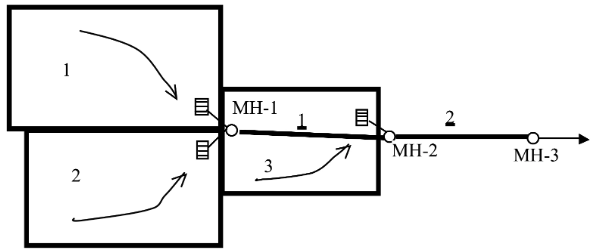
\includegraphics[width=6in]{DrainageSystemLayout.png} 
   \caption{Drainage System Schematic (Plan View)}
   \label{fig:drainage-schematic}
\end{figure}

Figure \ref{fig:contributingarea} lists drainage area information.
\begin{figure}[h!] %  figure placement: here, top, bottom, or page
   \centering
   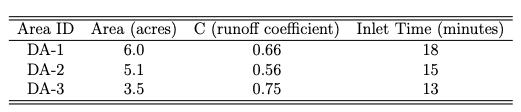
\includegraphics[width=4in]{ContributingArea.png} 
   \caption{Contributing Area Table}
   \label{fig:contributingarea}
\end{figure}

Figure \ref{fig:pipedata} shows a list of pipe connectivity, flow lengths, design slopes, and pipe roughness data.
\begin{figure}[h!] %  figure placement: here, top, bottom, or page
   \centering
   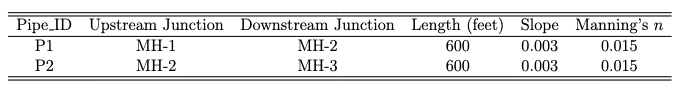
\includegraphics[width=4in]{PipeData.png} 
   \caption{Pipe Connectivity, Distances, and Slopes}
   \label{fig:pipedata}
\end{figure}

\clearpage

Figure \ref{fig:IDFequation} is the 10-year ARI intensity equation for the area, where $I$ is intensity in inches-per-hour, and $T_c$ is the averaging time, in minutes. Depending on the location in the system it may be just the local inlet time, or a time of concentration that includes upstream contributions and pipe travel time.

\begin{figure}[h!] %  figure placement: here, top, bottom, or page
   \centering
   
\includegraphics[width=6in]{Eqn1.png} 
   \caption{Drainage System Schematic (Plan View)}
   \label{fig:IDFequation}
\end{figure}

The allowable velocity at design flow is between 2 and 10 feet-per-second. The pipes are to be sized so they flow $\frac{1}{2}$ full at the design discharge.

Using the supplied problem data, and assuming the 10-year ARI is the design standard for the system, determine:

\begin{enumerate}
\item Determine the design flow rates in cfs for each pipe
\item Determine the associated pipe diameters in inches for both pipes.
\end{enumerate}


\end{document}  